\documentclass{amsart}
\usepackage{graphicx}
\graphicspath{{./}}
\usepackage{hyperref}
\usepackage{csvsimple}
\usepackage{longtable}
\usepackage{lscape}
\usepackage{epigraph}
\title{The Final Nail on the Coffin of Racial Supremacy Theories} 
\author{Zulfikar Moinuddin Ahmed}
\date{\today}
\begin{document}
\maketitle

\section{The Delicate Issues of Organising the Final Nail on Coffin of Racial Supremacy Theories}

Many years ago, I was moved by the great book of Stephen Jay Gould entitled {\em The Mismeasure of Man}.  For me this was a curious book and not central to my intellectual interests of the time either.  It might have been in New York when I was then married to the academic Natalia Brizuela.  I had many other things on my mind then.  I had absorbed some issues of British Colonialism in India then.  You have to understand that I was born in 1973 in Bengal, Northeast of India.  The Vietnam War had been going on for some years before my birth in neighboring countries.  The fall of Saigon happened in April 1975, when I had the privilege still of bein the only son of my parents;  in July my brother Feroze Alamgir Ahmed wud be born, and I would play with him for some days and ask my mother to return him to the hospital but would be shocked to learn that he was permanently going to consume my parents affection with more natural charm than myself.  Now before I speak of {\em racial} superiority issues, let me talk a little bit about my various deep psychological insecurities that developed from childhood.  I gave up playing chess altogether quite young because my brother was just much better at it than me.  I was much more internal than him, and was less social as well.  Now let's take a look at the map to see where all this was going on.

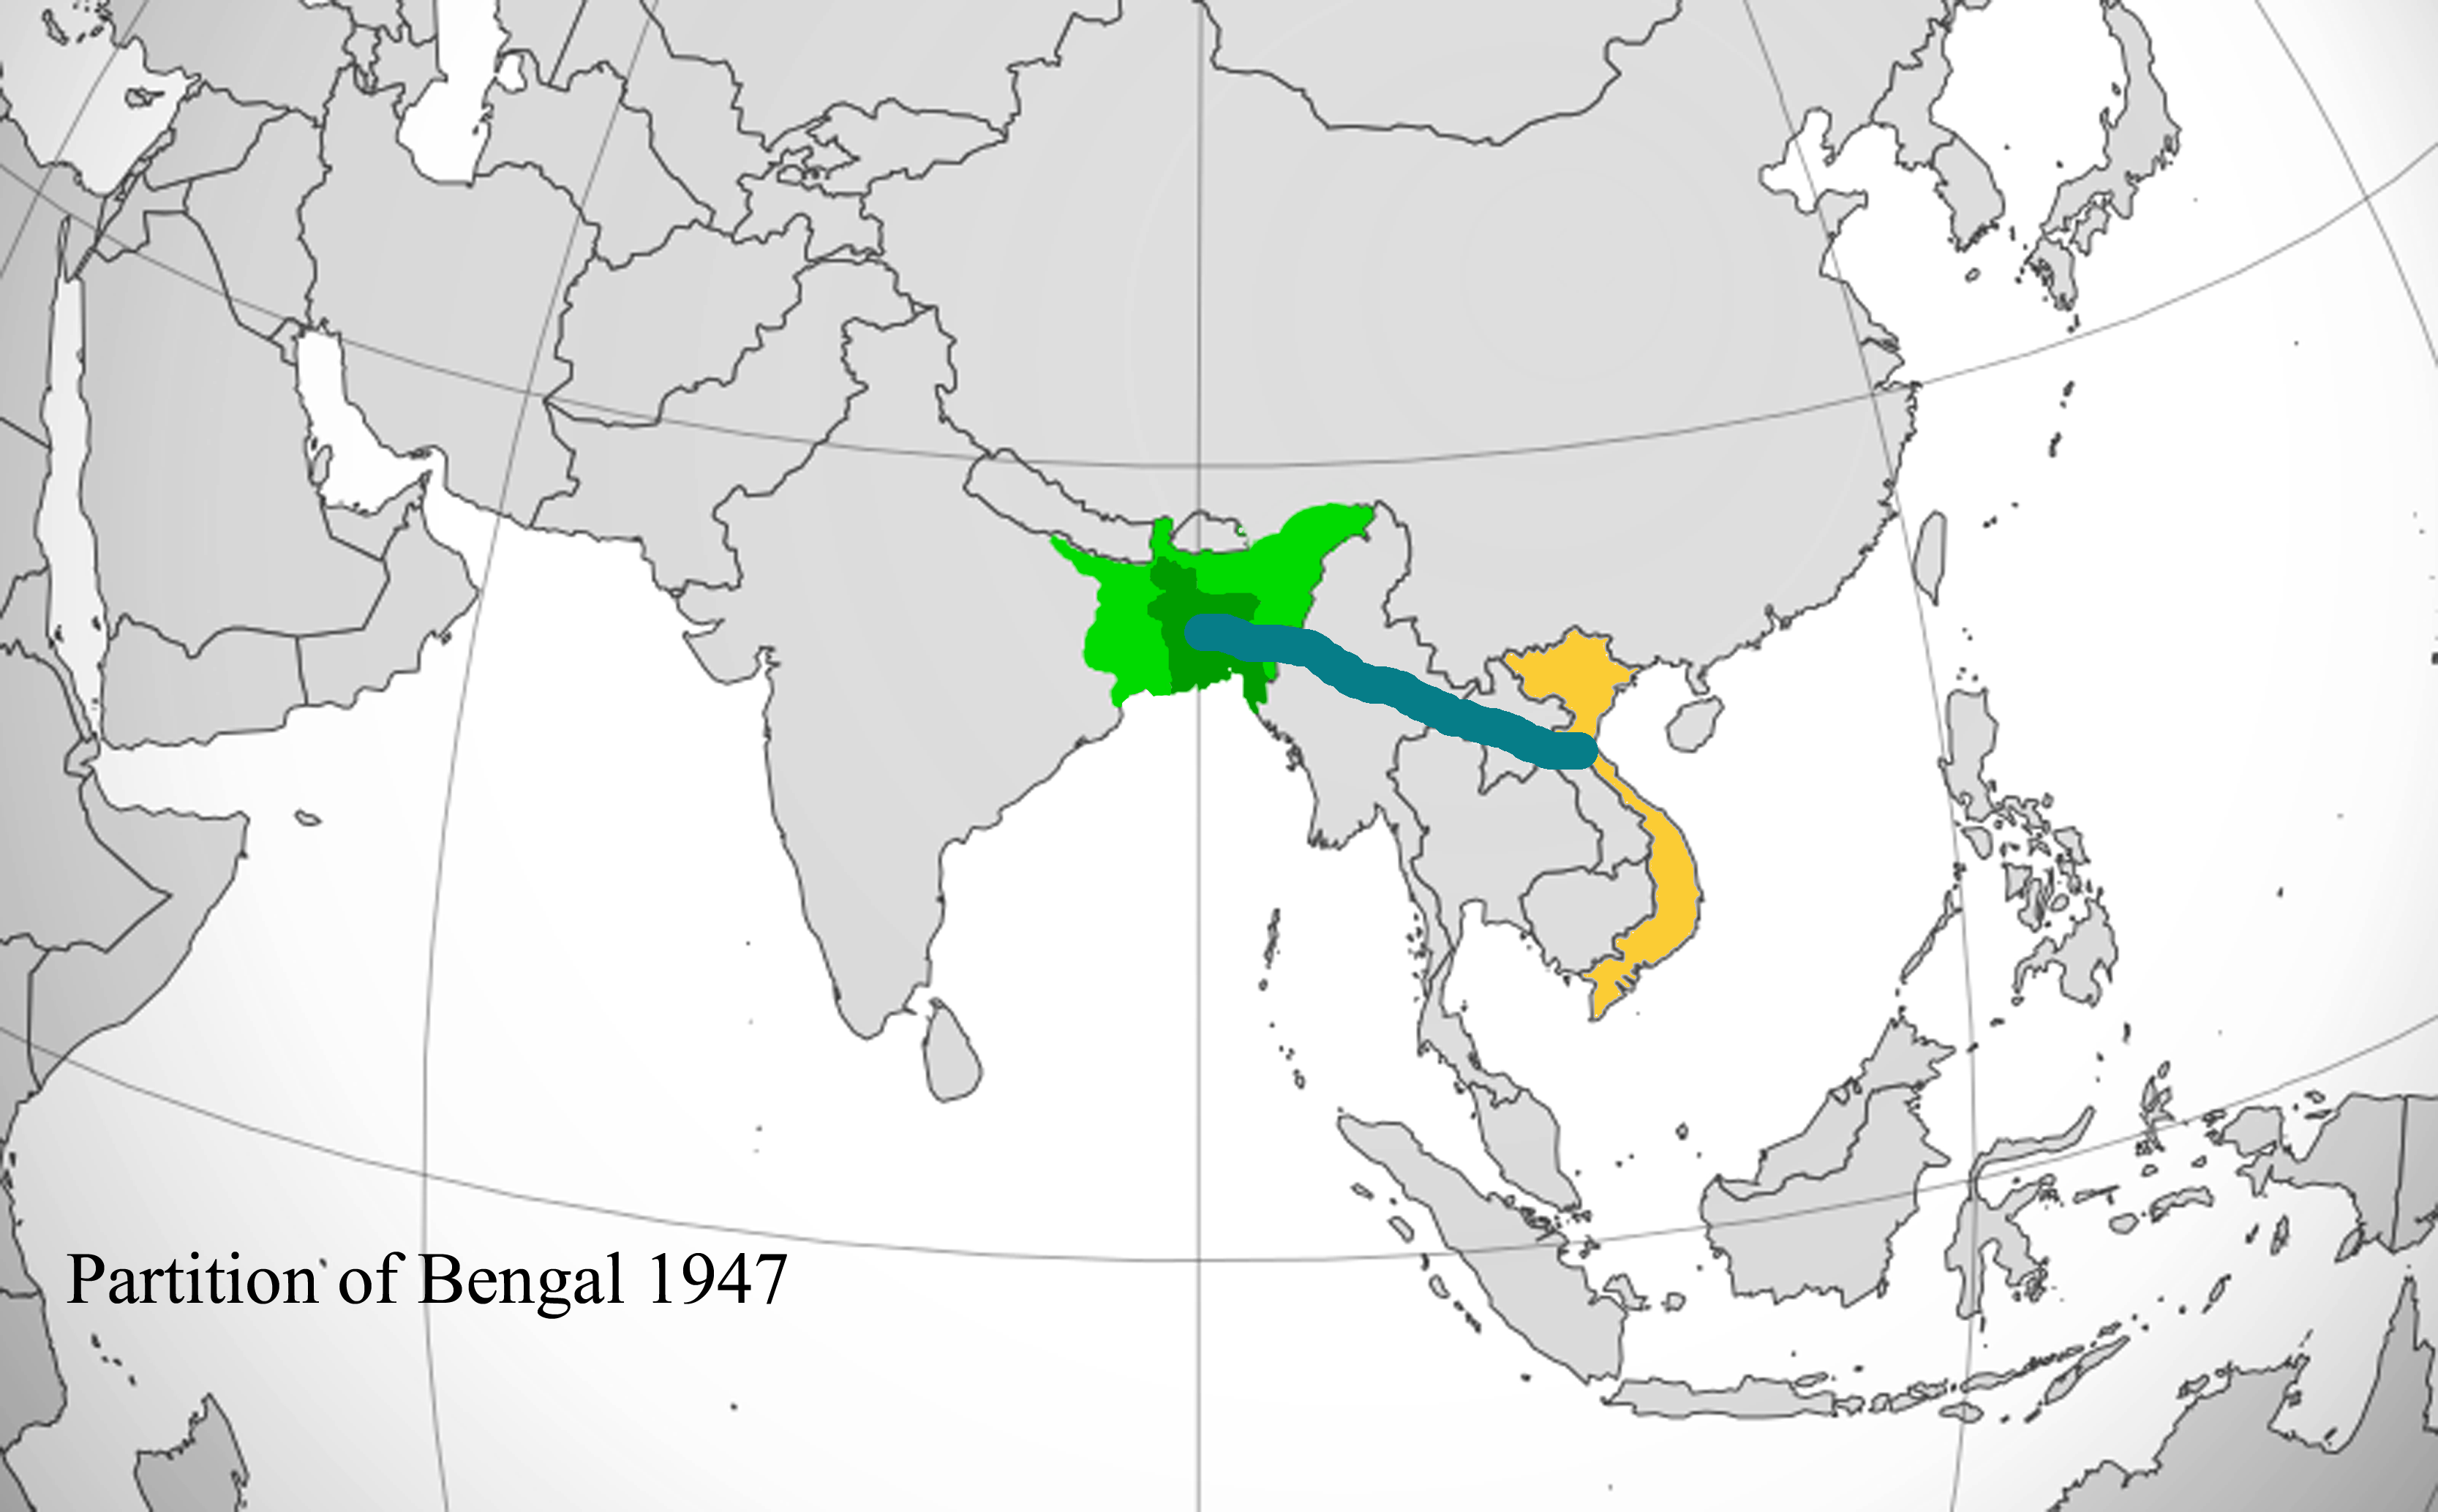
\includegraphics[scale=0.1]{bengal2.png}

I have marked Vietnam in yellow and drawn a line to Dhaka where I was born November 19 1973.  I am 100\% American of course, but I want to make clear to my readers the particular historical situation of my birth and ethnicity.  I am Bengali with 1/8 Persian from my father's mother's side.  My father's family is aritocratic all the way back to Vedic era 1750 BC.  This region was inhabited already in 500 BC with a literate Civilisation and then it was Vangala.  By the time I was born, India had become independent of England; India split into Pakistan; and Pakistan had splintered so the nation of Bangladesh was born several years before I was.  All these changes were, in the long run, quite irrelevant to me since I was far away in New York and think of my ancestry in India.

The point of all these details is to put my own ethnicity and race into the picture, to make clear that for me issues of ethnicity, race, inheritance, idenity and so on are quite serious and real issues and not matters of frivolity.  

I moved to America September of 1987, and began high school in a highly ethnically diverse are of Queens New York.  And I was too young to worry about ethnicity at all very much, and so I just got used to thinking of my Italian and Jewish and Guyanese and Irish and Hispanic and Black classmates as just people.  Like myself.  I was used to seeing different people of different ethnicities every day already by 1988.  This is very important.  For my mother, she had a history in Bengal.  My father never moved to America.  But for me, America became my home and my life was here.  I assimilated to white and Jewish and hispanic etc. multi-ethnic culture of New York.

\section{High School Valedictorian}

I went to John Adams High School, from late 1987 or early 1988 to 1991.  I was the Valedictorian of that year.  I was not white.  And in other years, there were white students who were valedictorian.  The school size was above 1,000 maybe 2,000.  There were many white students and many non-white.  I was very fortunate that Elizabeth Waltien, the coordinator of an accelerated Math-Science Institute discovered me one day while I was doing some service, and immediately gave me some tests and put me in Honours classes and took me under her wing, all the way to one of the most amazing letters of recommendation to Princeton University.  I am most grateful to her and keep her photograph still near me.
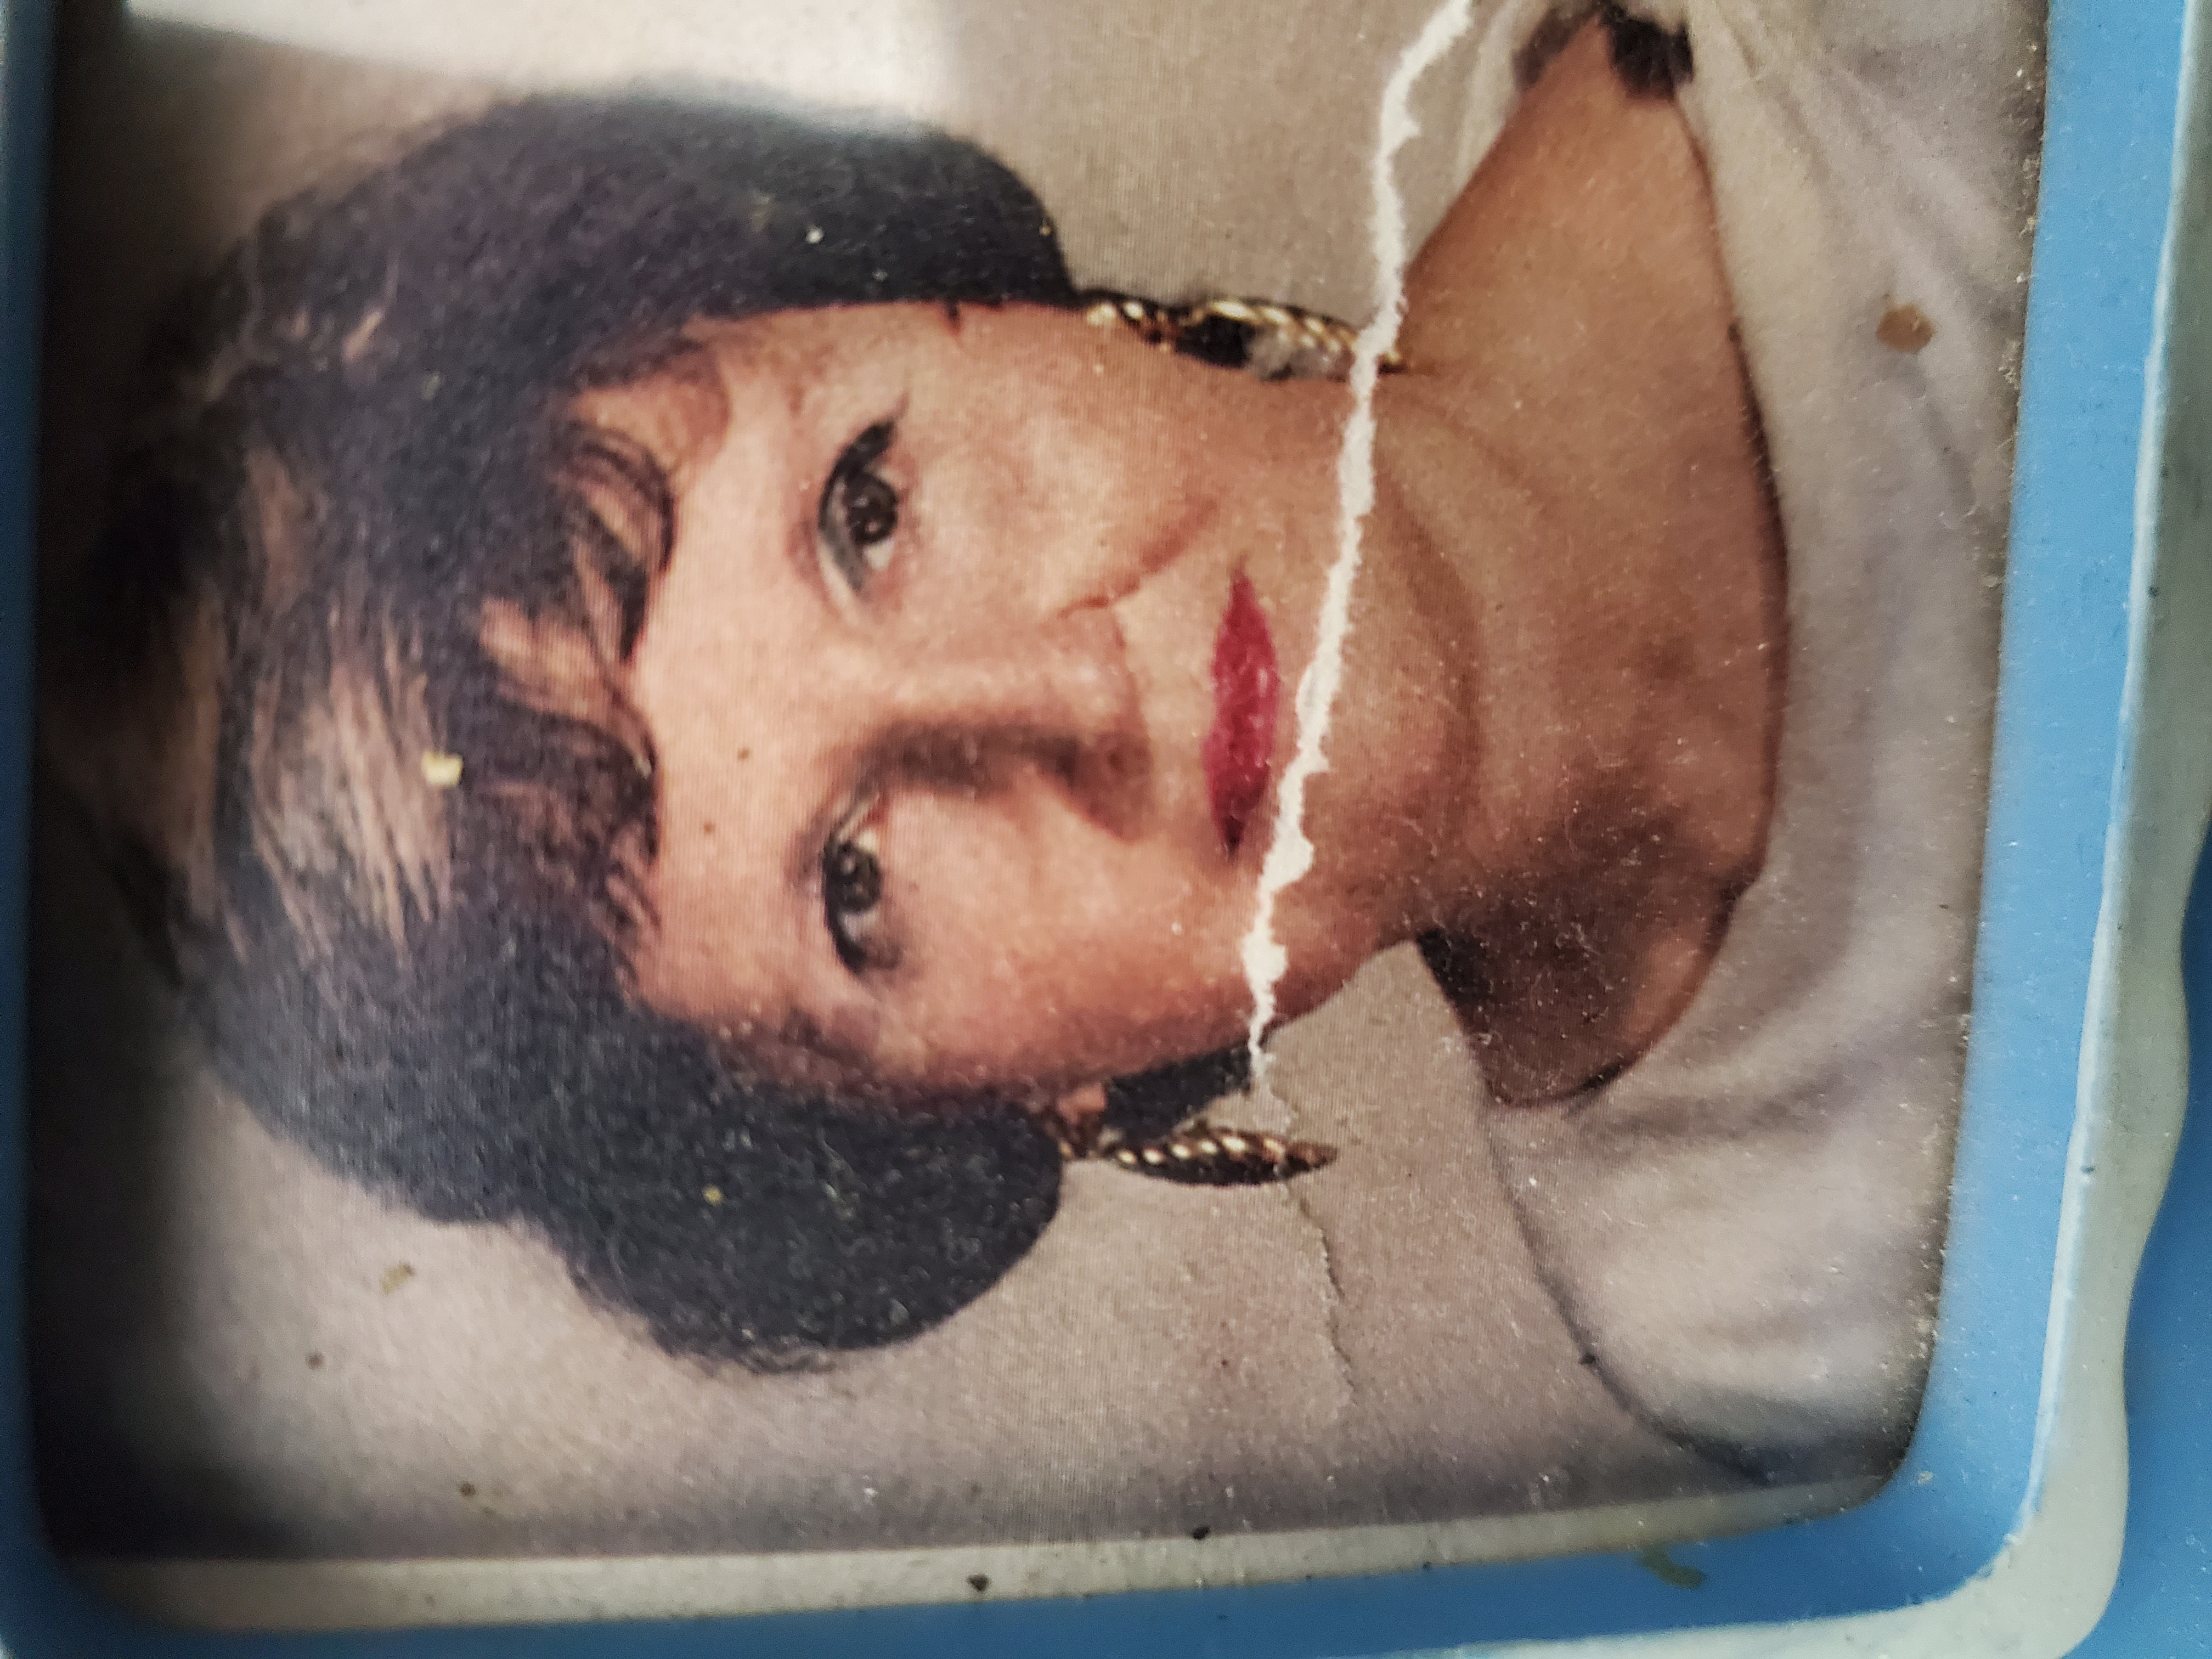
\includegraphics[angle=270,scale=0.1]{lys.jpg}
Throughout high school I had no racial feelings towards anyone.  I was treated with respect by my teachers, many of them Jewish or white, and I treated people with respect by and large.  I was a very good student, and I excelled in my classes.  I took Physics C and Calculus BC AP exams on my tenth grade and got 5 on both so I was assured to be on a Scientific track.  Lys Waltien was a tremendous inspiration; she had a spirituality that was deep and Catholic and she was a true Angel in my life.  I spent more time talking with her about philosophical issues after class than I even spent with many people my age.  She arranged for me to go to the Ohio State Ross Program for two summers.  There I bonded with people my age in an intimate setting of intense number theory and met Brian and Keith Conrad and many other great people like Josh Fishman, David Pollack, etc.  I assimilated there to music of Pink Floyd and Led Zeppelin and others.  I was extremely internal otherwise, and was deeply attached to Fyodor Dostoevsky and Franz Kafka, and was interested in literary issues already.  

All this biographical material will tell you that I was simply not racial at all.  I never sized anyone up by any ethnic criteria from an early age.  

I have had several white lovers, a black lover since graduation from Princeton in 1995, and I have never been convinced of multiple races of human beings.  The Single Human Race {\em conviction} for me arose naturally from life in America for me.  I was in fact surrounded always by intellectual elite; I still am, but there is nothing ethnic about my elitism really.  I am proud in a way of my 3000 year aristocracy, but that is an inner pride and not something that expresses itself in arrogance with random people.  Indeed, I think that cultivation and nobility is in the ability to treat people well.

\section{Why I Am Against Bengali-Supremacist World Order}

When I was very young, I was a sensitive boy, and loved little baby animals.  I had a pet chicken at my maternal grandmothers' house where my mom would drop me off.  She was a beautiful kind woman who was a published poet.  Bengali poetry is exquisitely beautiful and has a long history of thousands of years.  Bengali existed for as long as Ancient Greek as far as I know.  One day I was walking around in some garden or such and accidentally stepped on a little frog and killed it.  I was so ashamed and horrified by what I had done that I could not sleep all night and cried for the frog.  Years later, my ex-wife would be contemptuous of me when our kitten Rulfo died in New York and I did not go to Lehman Brothers for some days because I was heartbroken and was traumatised.  She told me she pitied me and so on.  I dislike mistreating people.  It would be so horrific if I lived in a Bengali Supremacist World Order.  All the beautiful people who I befriended would be distrustful that I would harm them, and people would look at me with consternation and fear rather than in an ordinary way.  I don't like the idea at all.  

I don't think most white people really like the idea of a White Supremacist World Order.  The population support for it in America is around 9\%, hardly significant enough to have any unity on the matter.  Now in the past, certainly this existed.  There are many accounts of horrific racially motivated slavery and mistreatment of people.

\section{The Right View of Superiority and Inferiority}

Human Race has had a {\em totally natural} scale of Superiority and Inferiority for millions of years.  It's understood by everyone.  Goodies and superior to Baddies.  I am a Goodie.  So I will obviously be superior to all the Baddies of the world, including Bill Gates. And I will show you some data later on that shows that in all Ethnicities roughly 95\% of all people are good, so the Baddies of Human Race form a minority of less than 5\%.  All Goodies are going to be Superior to all Baddies.  Ethnic Superiority is just wrong and misguided, because only 6.5\% to 9.5\% of human morality varies with ethnicity.  All superiority is really about moral character, and so Ethnic Superiority is impossible.

\section{Objective Analysis of Ethnicity Independence of Human Morals}

The universal human moral nature that is ethnicity-independent is my discovery, and one of my greatest discoveries.  It is such a profound discovery that I feel that it is Fate that propels me forward to end all ethnic strife on Earth, and that this, among others, was the purpose of my birth on Earth.  

In a previous note, I conducted a paired t-test for ethnicity pairs and found strong evidence that as vectors the 10-dimensional probability vectors are statistically indistinguishable.

Here I provide you with the visual display of the probability densities that gives us compelling evidence that these distributions are minor perturbations of each other and are not significantly different.


\section{Line Graphs}

\includegraphics[scale=0.7]{q177.jpeg}

\includegraphics[scale=0.7]{q178.jpeg}


\includegraphics[scale=0.7]{q179.jpeg}

\includegraphics[scale=0.7]{q180.jpeg}

\includegraphics[scale=0.7]{q181.jpeg}

\includegraphics[scale=0.7]{q182.jpeg}

\includegraphics[scale=0.7]{q183.jpeg}

\includegraphics[scale=0.7]{q184.jpeg}

\includegraphics[scale=0.7]{q185.jpeg}

\includegraphics[scale=0.7]{q186.jpeg}

\includegraphics[scale=0.7]{q187.jpeg}

\includegraphics[scale=0.7]{q188.jpeg}

\includegraphics[scale=0.7]{q189.jpeg}

\includegraphics[scale=0.7]{q190.jpeg}

\includegraphics[scale=0.7]{q191.jpeg}

\includegraphics[scale=0.7]{q192.jpeg}

\includegraphics[scale=0.7]{q193.jpeg}

\includegraphics[scale=0.7]{q194.jpeg}

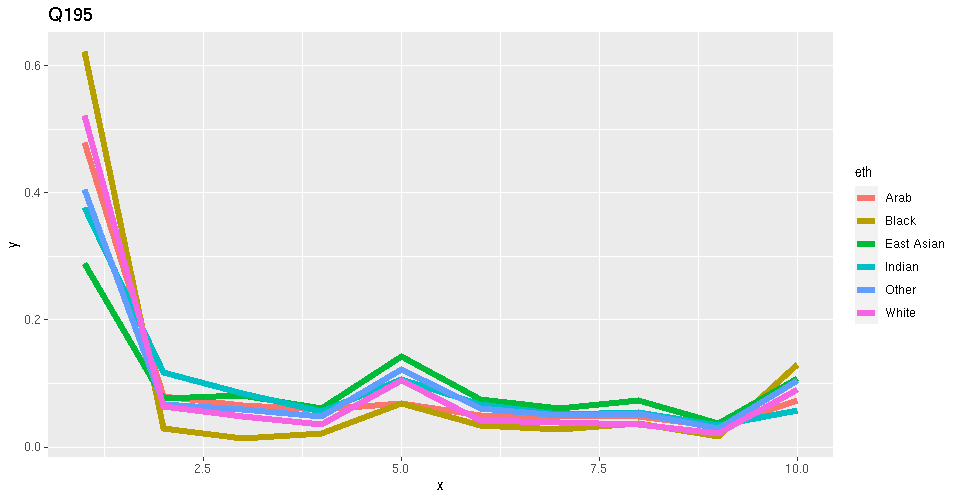
\includegraphics[scale=0.7]{q195.jpeg}

\section{Precise Variation Explained By Ethnicity}

We consider a measure that is like $R^2$ now to tabulate the effect of ethnicity on moral value distribution.  We compute this as residual sum of squares divided by total sum of squares wih respect to the mean mean curve over ethnicities.

% latex table generated in R 4.0.3 by xtable 1.8-4 package
% Sat May  8 00:26:41 2021
\begin{table}[ht]
\centering
\begin{tabular}{rlr}
  \hline
 & eth & explained \\ 
  \hline
1 & Arab & 4.82 \\ 
  2 & Black & 3.75 \\ 
  3 & East Asian & 4.85 \\ 
  4 & Indian & 7.73 \\ 
  5 & Other & 1.89 \\ 
  6 & White & 6.07 \\ 
   \hline
\end{tabular}
\end{table}

We get values roughly between 2-8\%.  This is reasonable and fairly small, and quite mysterious.  Across the world, we {\em share} almost identical moral value preferences with ethnic variation in this range 2-8\%.




\end{document}
